% anhang.tex
\chapter{Visualisierung der Samtfleckenkrankheit}
\label{anahngd}
\begin{figure}[h!]
	\centering
	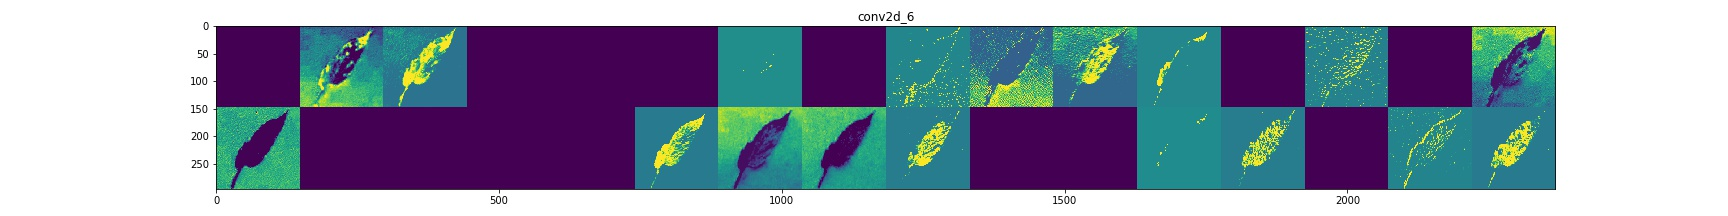
\includegraphics[width=\textwidth]{visualisierungen/leaf_mold/activation/mold0.JPG}
	\caption{Visualisierung der Aktivierungswerte in der ersten Faltungschicht von der Samtfleckenkrankheit (eigene Darstellung).}
	\label{}
\end{figure}

\begin{figure}[h!]
	\centering
	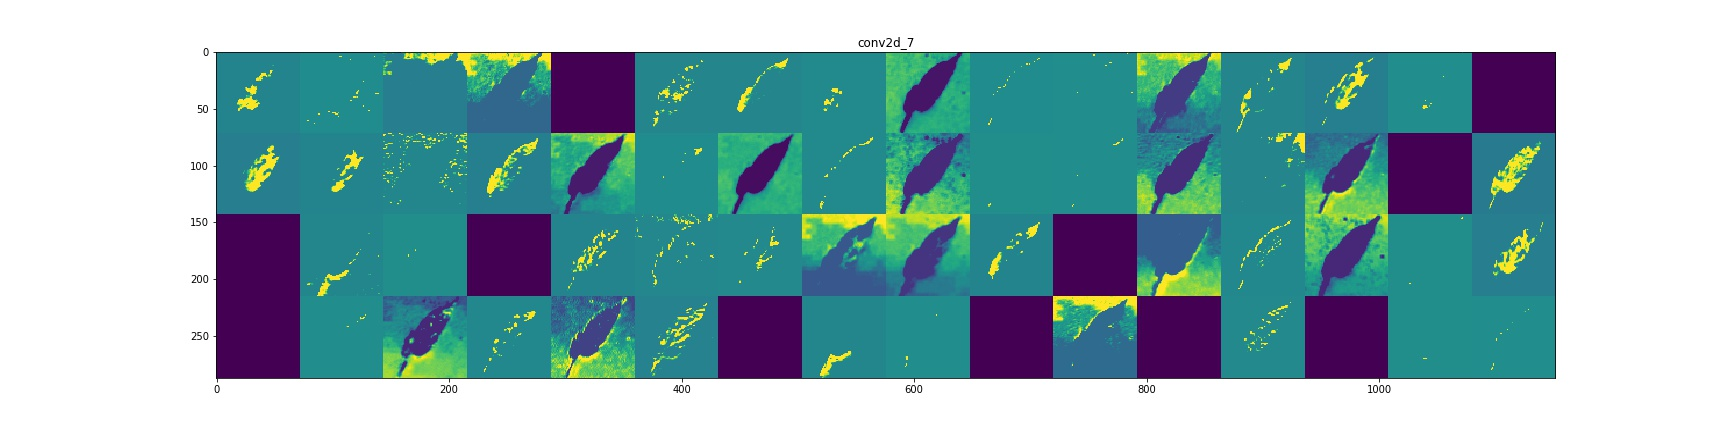
\includegraphics[width=\textwidth]{visualisierungen/leaf_mold/activation/mold3.JPG}
	\caption{Visualisierung der Aktivierungswerte in der zweiten Faltungschicht von der Samtfleckenkrankheit (eigene Darstellung).}
	\label{}
\end{figure}

\begin{figure}[h!]
	\centering
	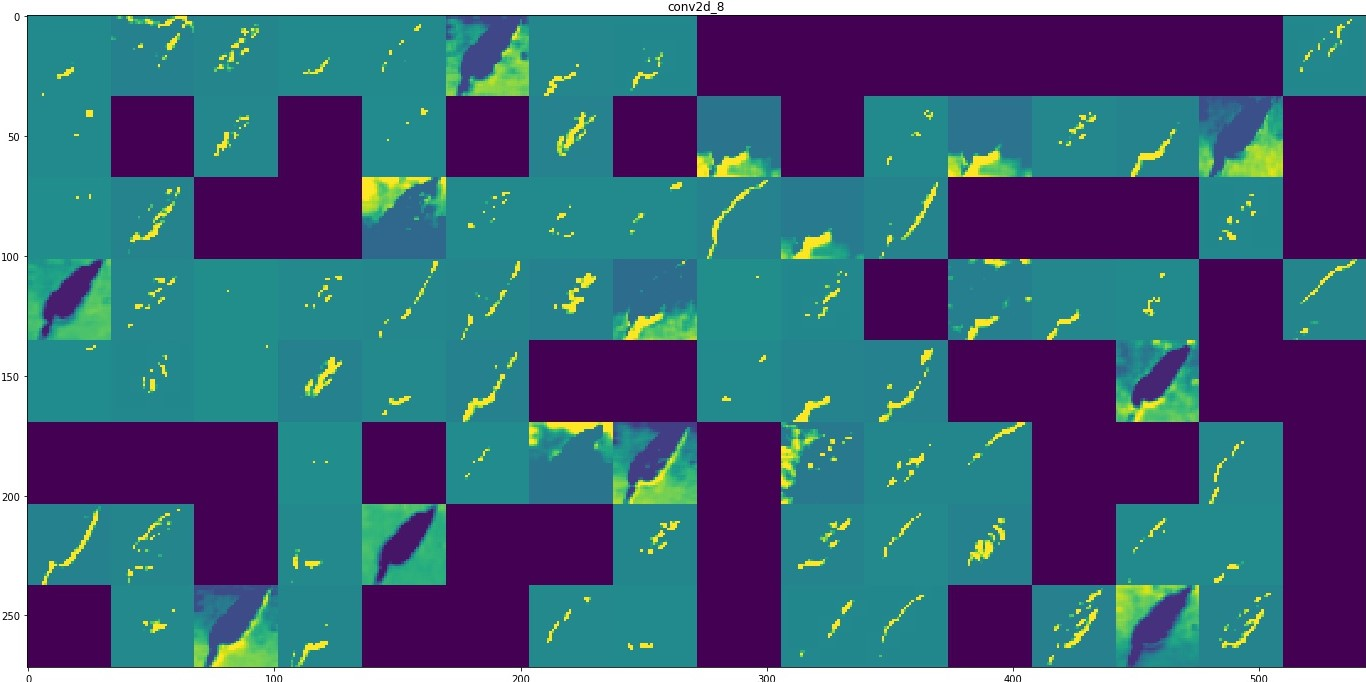
\includegraphics[width=\textwidth]{visualisierungen/leaf_mold/activation/mold6.JPG}
	\caption{Visualisierung der Aktivierungswerte in der dritten Faltungschicht von der Samtfleckenkrankheit (eigene Darstellung).}
	\label{}
\end{figure}

\begin{figure}[h!]
	\centering
	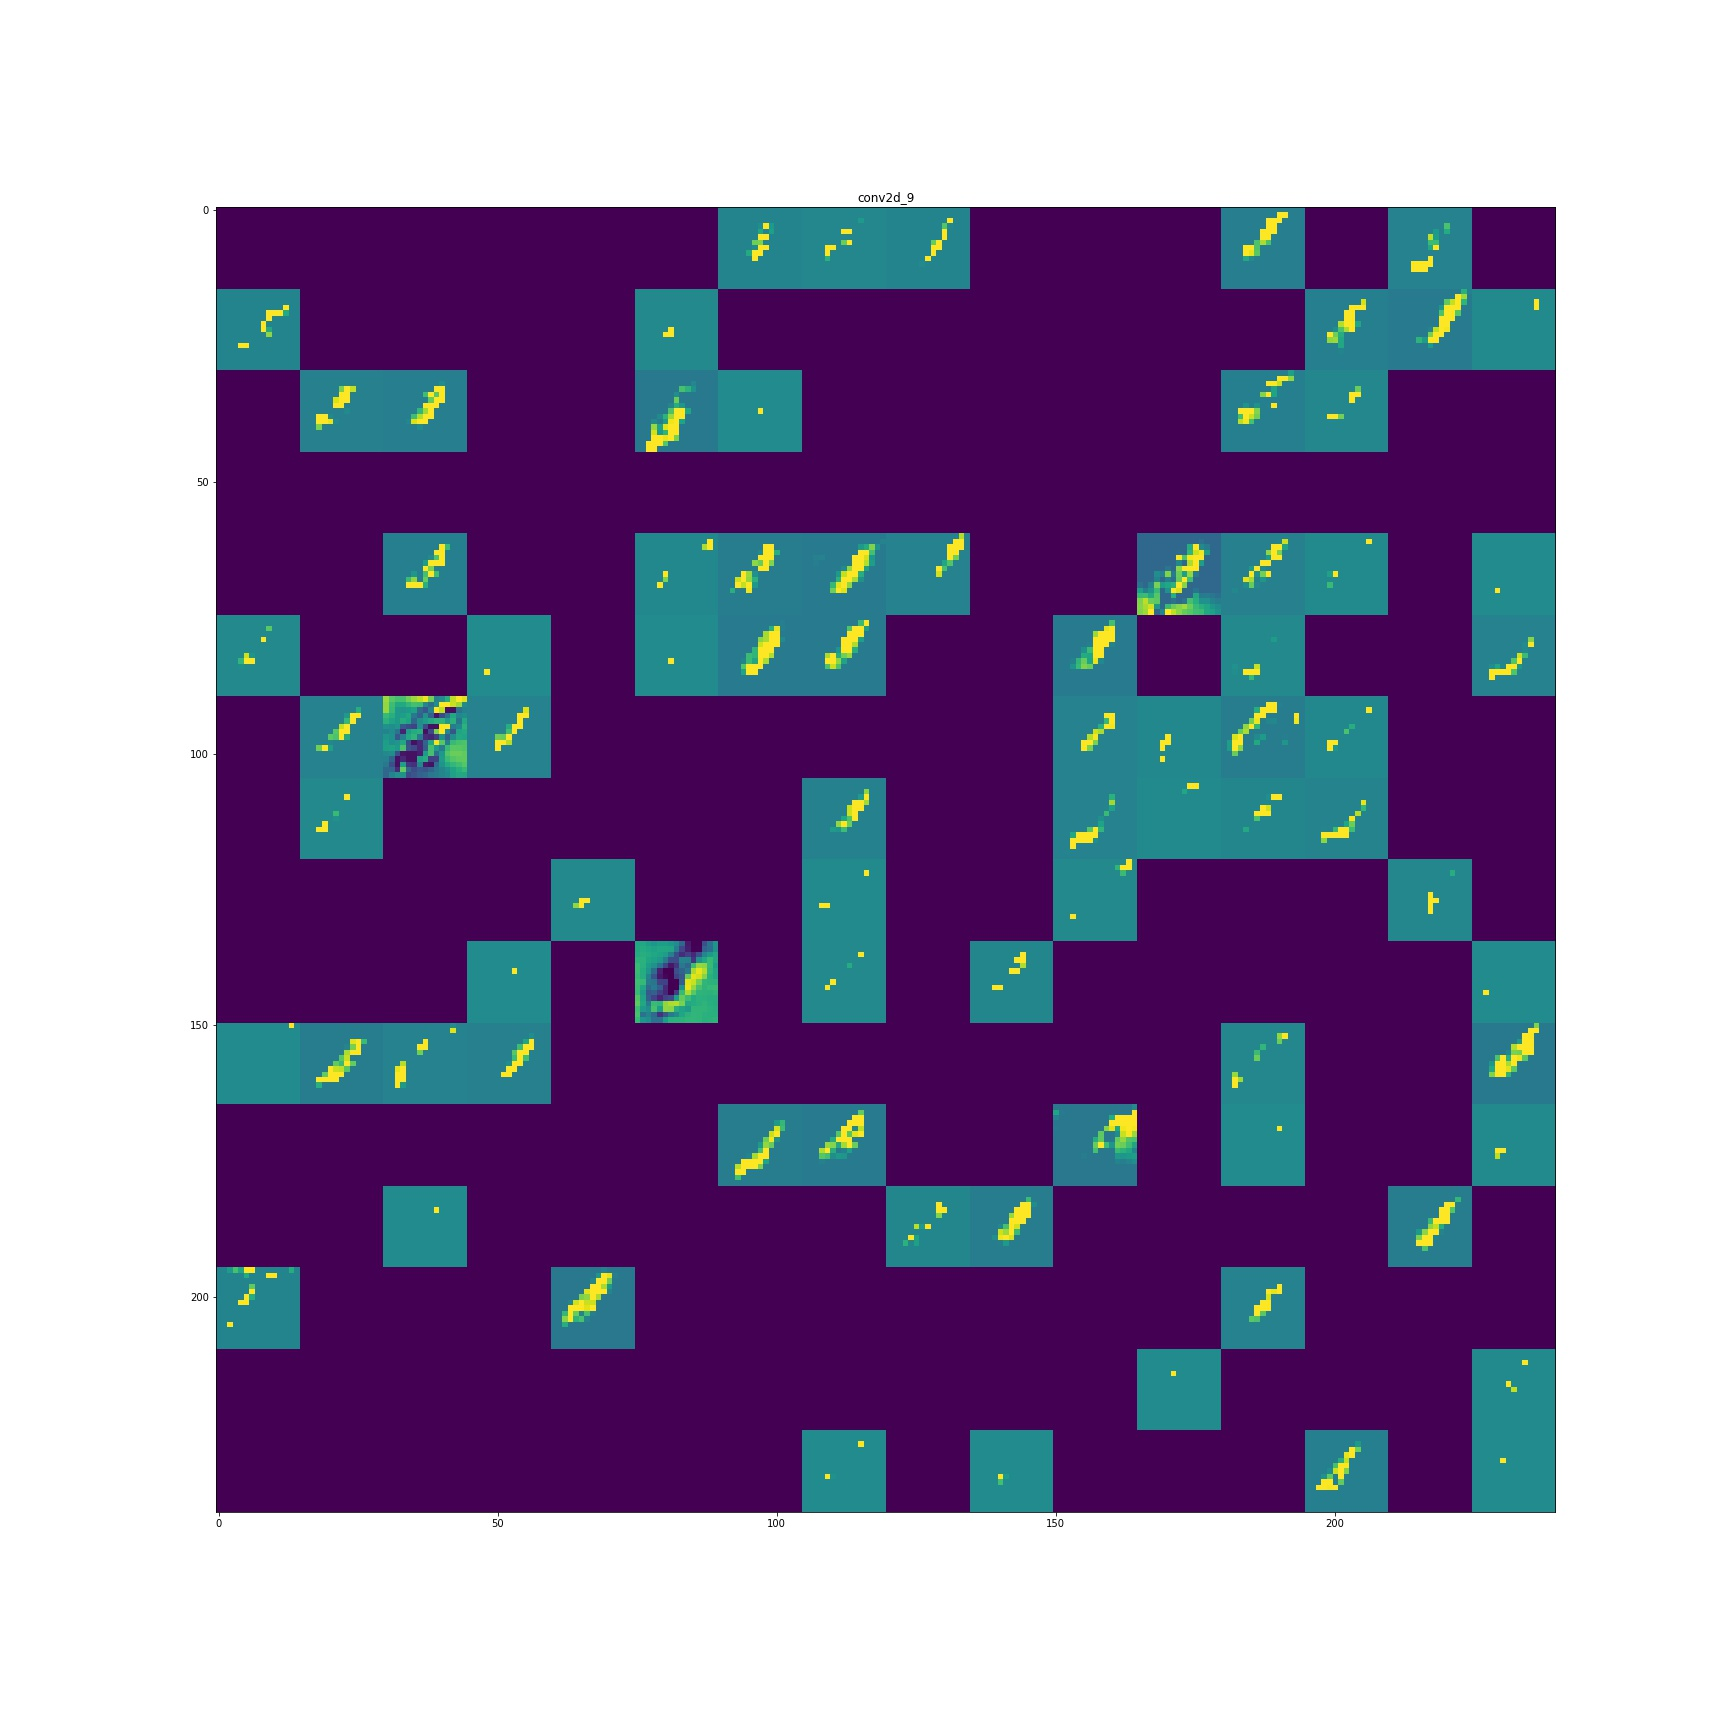
\includegraphics[width=\textwidth]{visualisierungen/leaf_mold/activation/mold8.JPG}
	\caption{Visualisierung der Aktivierungswerte in der vierten Faltungschicht von der Samtfleckenkrankheit (eigene Darstellung).}
	\label{mold8_anhang}
\end{figure}

\begin{figure}[h!]
	\centering
	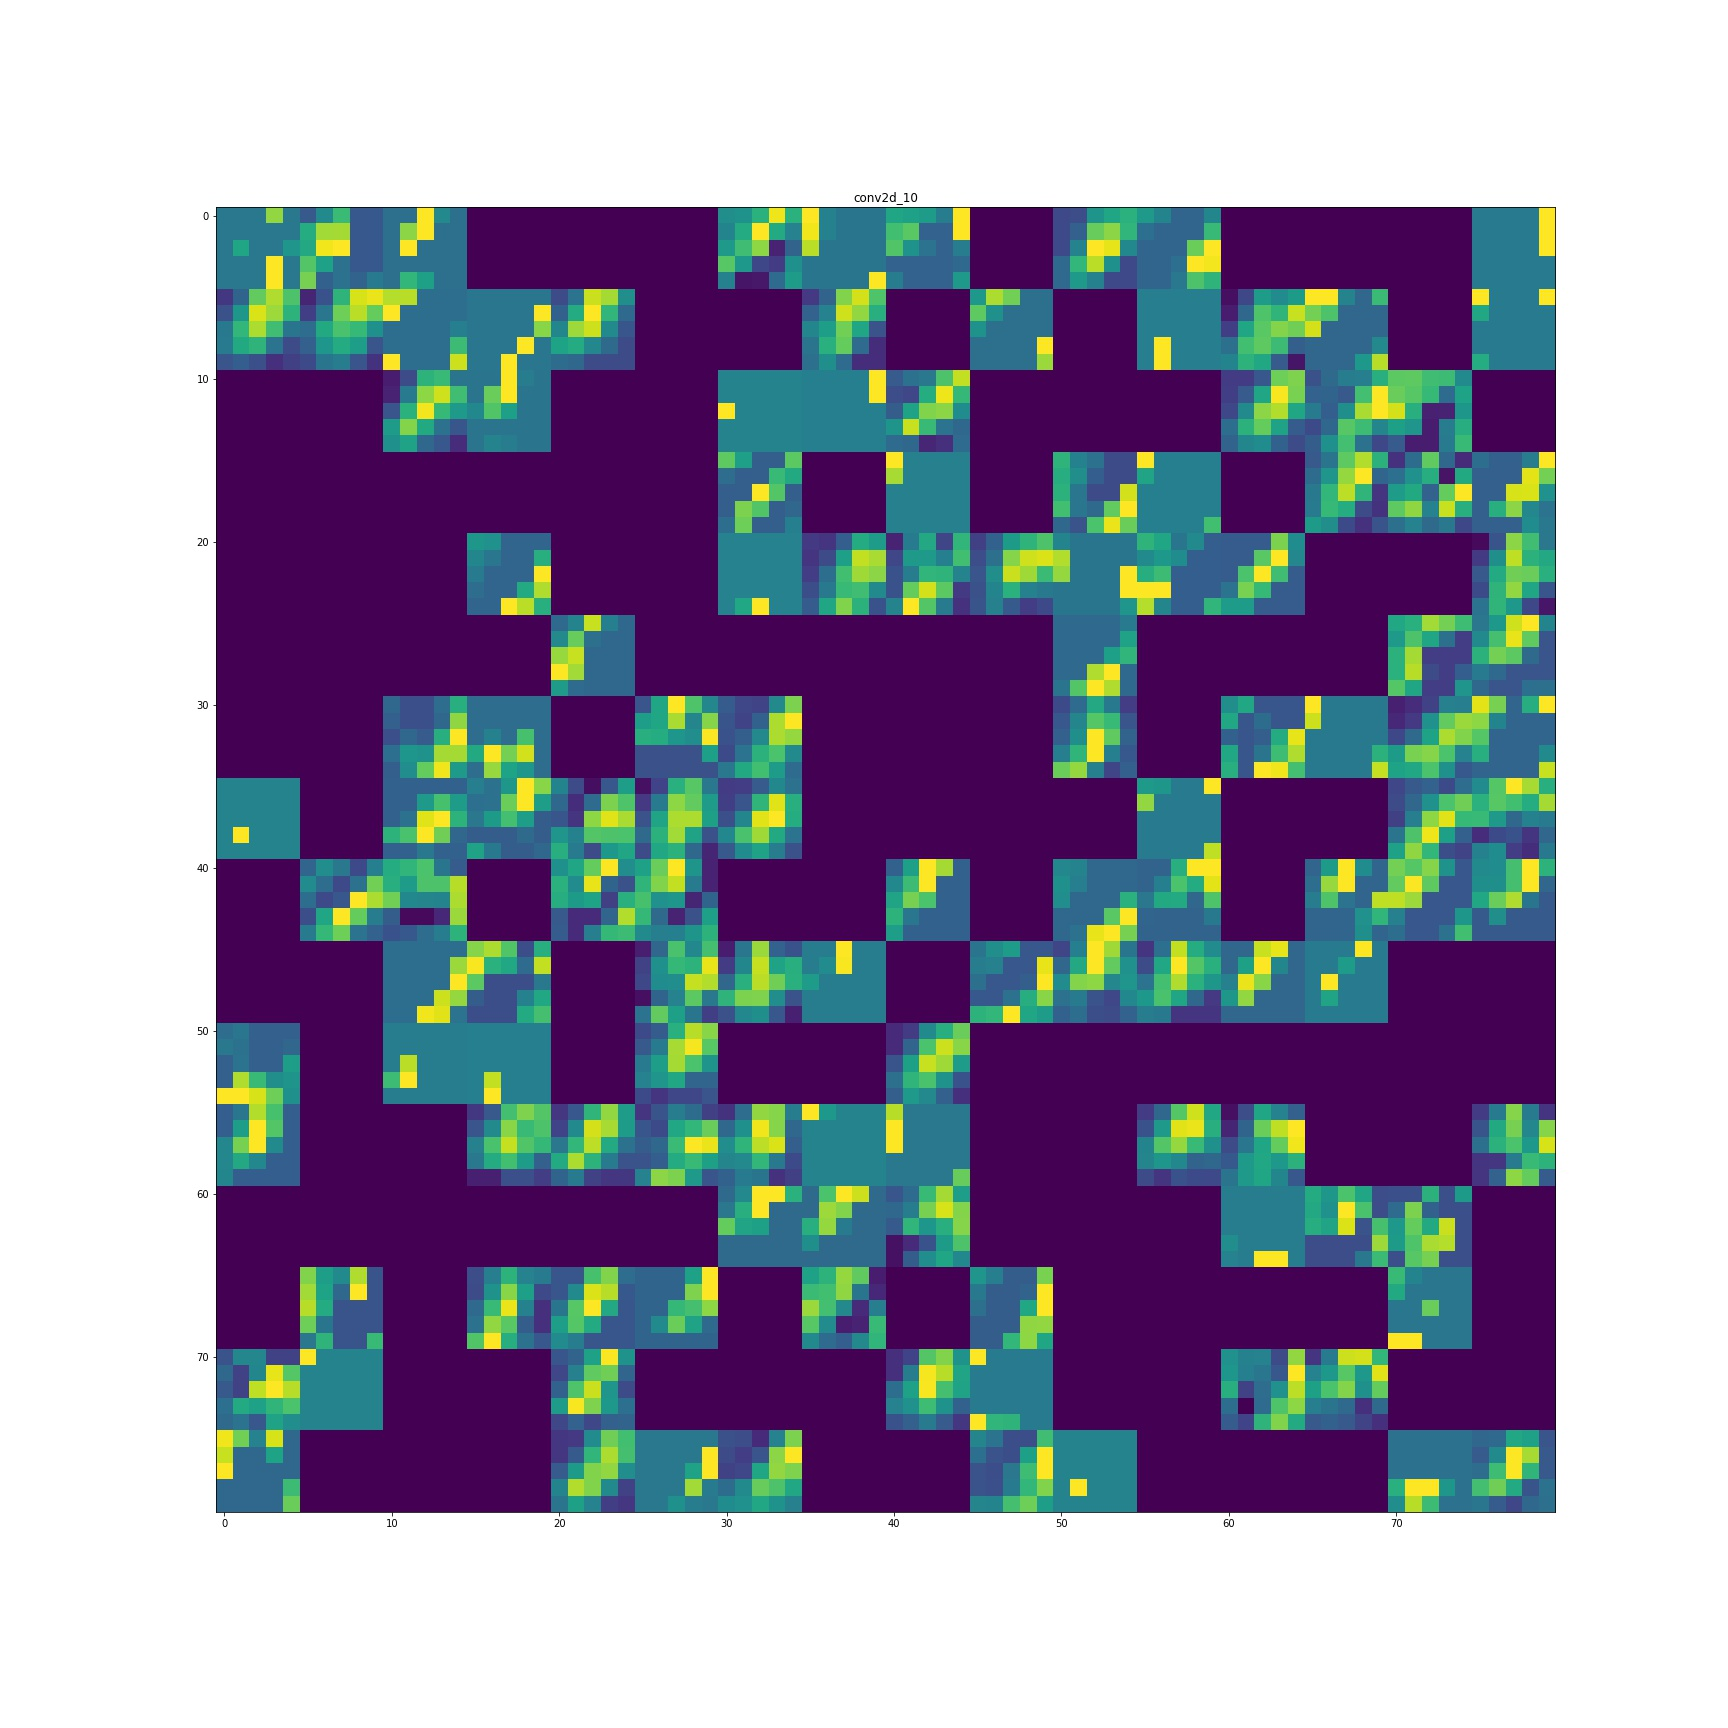
\includegraphics[width=\textwidth]{visualisierungen/leaf_mold/activation/mold10.JPG}
	\caption{Visualisierung der Aktivierungswerte in der fünften Faltungschicht von der Samtfleckenkrankheit (eigene Darstellung).}
	\label{}
\end{figure}


%%%%%%%%%%%%%%%%%%%%%%%%%%%%%%%%%%%%%%%%%%%%%%

\begin{figure}[h!]
	\centering
	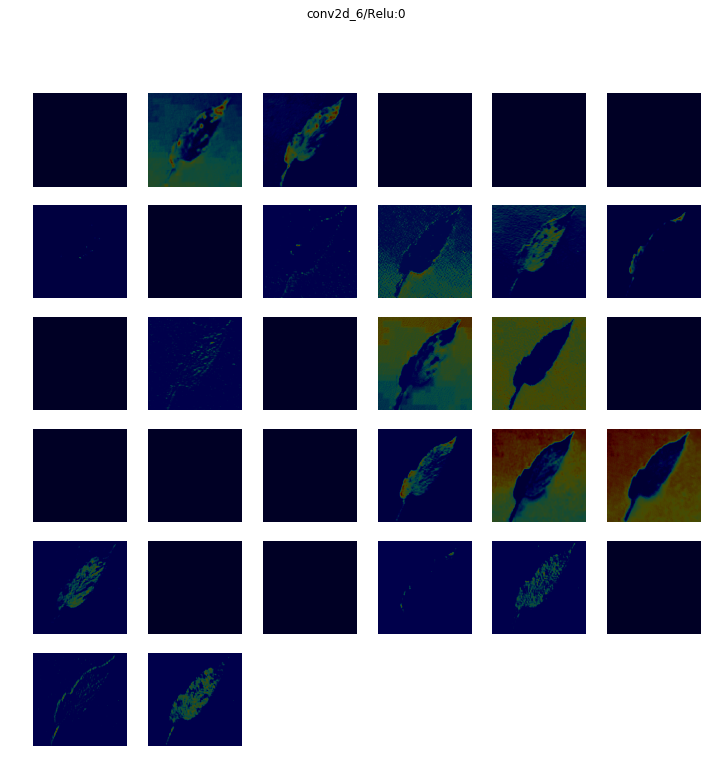
\includegraphics[width=\textwidth]{visualisierungen/leaf_mold/heatmap_mit/conv2d_6.png}
	\caption{Visualisierung der Aktivierungswerte als Heatmap in der ersten Faltungschicht von der Samtfleckenkrankheit (eigene Darstellung).}
	\label{}
\end{figure}

\begin{figure}[h!]
	\centering
	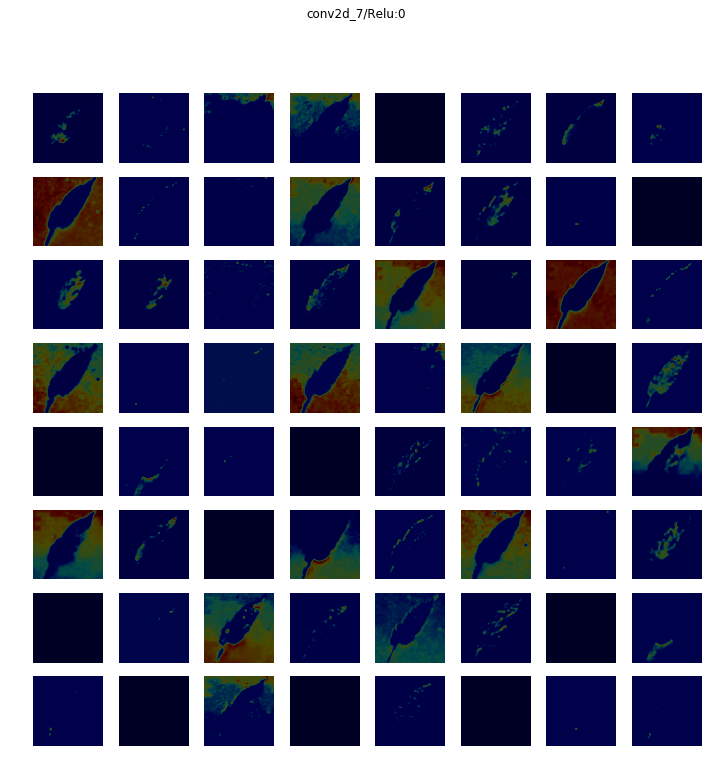
\includegraphics[width=\textwidth]{visualisierungen/leaf_mold/heatmap_mit/conv2d_7.png}
	\caption{Visualisierung der Aktivierungswerte als Heatmap in der zweiten Faltungschicht von der Samtfleckenkrankheit (eigene Darstellung).}
	\label{}
\end{figure}

\begin{figure}[h!]
	\centering
	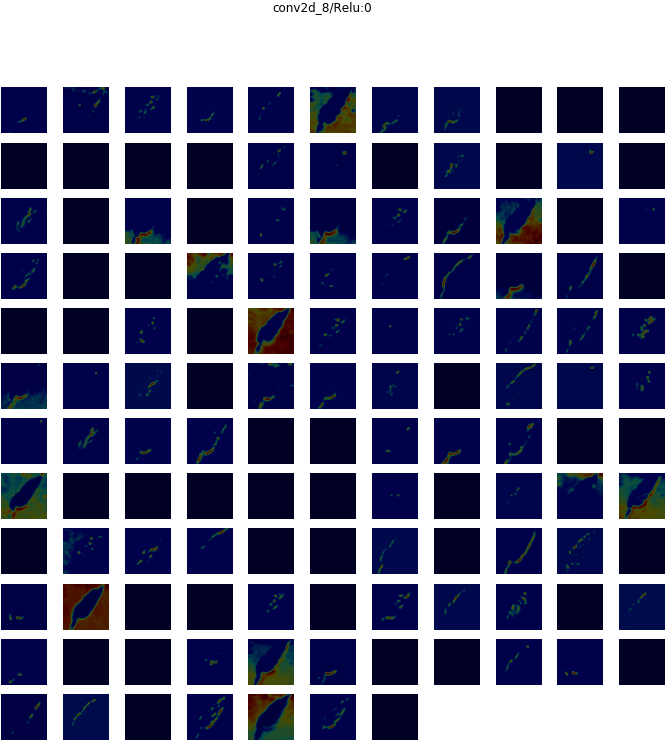
\includegraphics[width=\textwidth]{visualisierungen/leaf_mold/heatmap_mit/conv2d_8.png}
	\caption{Visualisierung der Aktivierungswerte als Heatmap in der dritten Faltungschicht von der Samtfleckenkrankheit (eigene Darstellung).}
	\label{}
\end{figure}

\begin{figure}[h!]
	\centering
	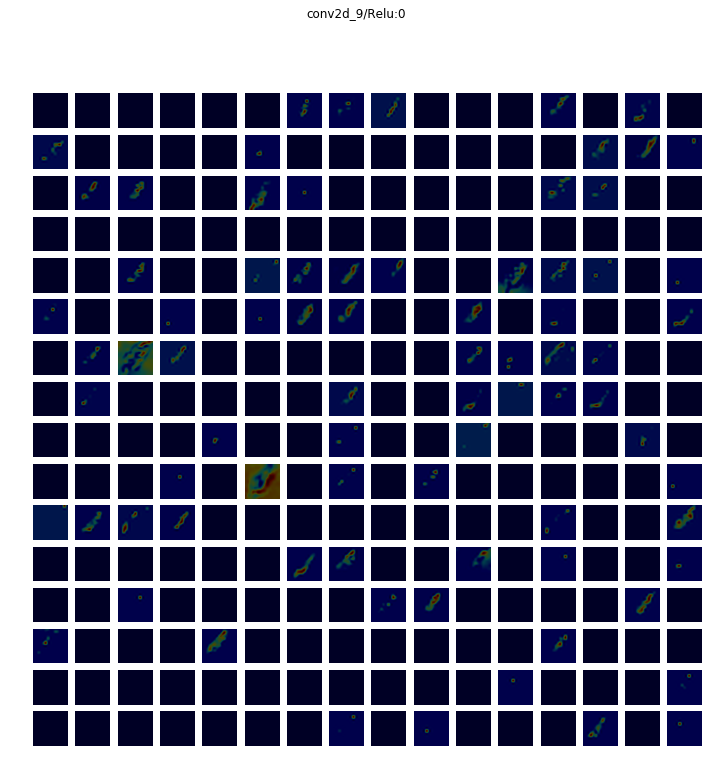
\includegraphics[width=\textwidth]{visualisierungen/leaf_mold/heatmap_mit/conv2d_9.png}
	\caption{Visualisierung der Aktivierungswerte als Heatmap in der vierten Faltungschicht von der Samtfleckenkrankheit (eigene Darstellung).}
	\label{}
\end{figure}

\begin{figure}[h!]
	\centering
	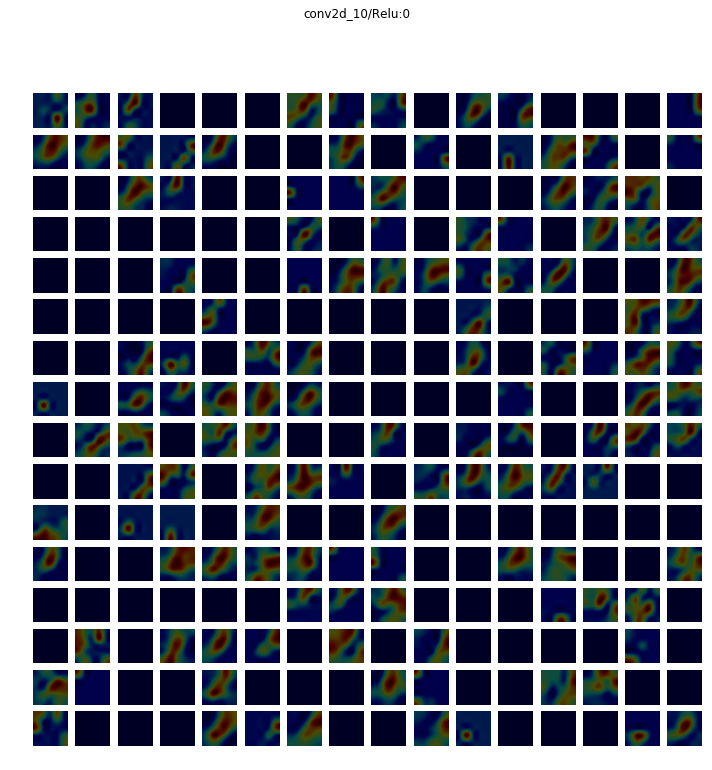
\includegraphics[width=\textwidth]{visualisierungen/leaf_mold/heatmap_mit/conv2d_10.png}
	\caption{Visualisierung der Aktivierungswerte als Heatmap in der fünften Faltungschicht von der Samtfleckenkrankheit (eigene Darstellung).}
	\label{}
\end{figure}
